% ================================================================================
% E-AI Tutorial Slides
% Filename: lec16.tex
%
% Roland Potthast 2025/2026
% Licence: CC-BY4.0
% ================================================================================
\documentclass[aspectratio=169]{beamer}

% --- Load lecture macros --------------------------------------------------------
% =================================================================================
% E-AI Tutorial Tex Macros for Slides
% Filename: lec_macros.tex
% 
% DWD, Roland Potthast 2025/2026
% Licence: CC-BY4.0
% =================================================================================

% --------------------------------------------------------------------------------
% Packages
% --------------------------------------------------------------------------------
\usepackage[T1]{fontenc}
\usepackage{lmodern}
\usepackage{graphicx}
\usepackage{tikz}
\usepackage{ragged2e}
\usepackage{xcolor}
\usepackage{tcolorbox}
\tcbuselibrary{listings,skins,breakable}
\usepackage{listings}
\tcbuselibrary{breakable}
\usepackage{graphicx}
\usepackage{fancybox}
\usepackage{xcolor}
\usepackage{xparse}
\usepackage{tikz}
\usepackage{fontawesome5}
\usepackage{amsmath,amssymb}
\usepackage{hyperref}
\usepackage{adjustbox}
% in lec_macros.tex (or lec17.tex preamble)
\usetikzlibrary{calc}

% Shortcuts for number sets
\newcommand{\R}{\mathbb{R}}

\usetikzlibrary{positioning,arrows.meta}


% --------------------------------------------------------------------------------
% Beamer setup
% --------------------------------------------------------------------------------
\setbeamertemplate{navigation symbols}{}
\setbeamercolor{background canvas}{bg=white}
\usepackage{pifont}
\usepackage{xcolor}

\usepackage{pifont}
\newcommand{\mdcheck}{\textcolor{green!70!black}{\ding{51}}}

% --------------------------------------------------------------------------------
% Colours
% --------------------------------------------------------------------------------
\definecolor{DWDblue}{RGB}{0,68,136}
\setbeamercolor{DWDrule}{fg=DWDblue}
\definecolor{codegreen}{rgb}{0.0, 0.5, 0.0} % Dark green for comments
\definecolor{codeblue}{rgb}{0.0, 0.2, 0.6} % Muted dark blue for keywords
\definecolor{codered}{rgb}{0.6, 0.1, 0.1}  % Muted red for strings
\definecolor{codegray}{rgb}{0.4, 0.4, 0.4} % Gray for numbers and operators
\definecolor{backcolor}{rgb}{0.97, 0.97, 0.97} % Very light gray background
\definecolor{lightblue}{RGB}{220, 230, 241} % Light blue for alternating rows
\definecolor{headerblue}{RGB}{180, 200, 230} % Slightly darker blue for headers
\definecolor{appendixblue}{RGB}{200, 220, 240} % Blue for appendix header
\definecolor{darkgreen}{RGB}{0,110,80}

\newcommand{\y}[1]{%
\colorbox{yellow!50}{#1}%
}\newcommand{\g}[1]{%
\colorbox{darkgreen!30}{#1}%
}
\newcommand{\red}{\color{red}}

% --------------------------------------------------------------------------------
% 
% --------------------------------------------------------------------------------
\newcommand{\rtext}[1]{{\color{red}#1}}

\newenvironment{tightmath}{
  \setlength{\abovedisplayskip}{3pt}
  \setlength{\belowdisplayskip}{3pt}
  \setlength{\abovedisplayshortskip}{2pt}
  \setlength{\belowdisplayshortskip}{2pt}
}{}

% --------------------------------------------------------------------------------
% Fonts
% --------------------------------------------------------------------------------
\setbeamerfont{title}{size=\Large,series=\bfseries}
\setbeamerfont{normal text}{size=\normalsize}

% --------------------------------------------------------------------------------
% Slide metadata
% --------------------------------------------------------------------------------
\newcommand{\LectureAuthor}{Roland Potthast}
\newcommand{\LectureYear}{2025--2026}

% --------------------------------------------------
% Header with logos
% --------------------------------------------------
\newcommand{\toplogos}{
  \noindent
  \vspace*{-5mm}
  \begin{minipage}{\textwidth}
    \raisebox{-0.5\height}{\includegraphics[height=1cm]{../../images/img00/ecmwf.png}}
    \hfill
    \raisebox{-0.5\height}{\includegraphics[height=0.9cm]{../../images/img00/university-of-reading-logo-vector.png}}
    \hfill
    \raisebox{-0.5\height}{\includegraphics[height=0.7cm]{../../images/img00/DWD-Logo_2013.svg.png}}
  \end{minipage}

  \vspace{-1mm}
\noindent
\begin{tikzpicture}
  \draw[DWDblue, line width=0.6pt] (0,0) -- (\textwidth,0);
\end{tikzpicture}
  \vspace{-3mm}
}

% --------------------------------------------------
% Title macro
% --------------------------------------------------
\newcommand{\mytitle}[1]{%
  {\usebeamerfont{title}\normalsize\color{DWDblue} #1}%
  \vspace{2mm}
}

% --------------------------------------------------
% Two-column layout macro
% --------------------------------------------------
\newcommand{\mycolumns}[2]{%
  \begin{columns}[T,totalwidth=\textwidth]
    \begin{column}{0.48\textwidth}
      \justifying
      #1
    \end{column}
    \begin{column}{0.48\textwidth}
      #2
    \end{column}
  \end{columns}
}

\makeatletter
% --------------------------------------------------------------------------------
% Footer: line + author | lecture | year | slide number
% --------------------------------------------------------------------------------
\setbeamertemplate{footline}{
  \leavevmode

% --- horizontal line above footer --------------------------------------------
\hbox to \paperwidth{%
  \hskip\beamer@leftmargin
  \begin{tikzpicture}
    \draw[DWDblue, line width=0.6pt]
      (0,0) --
      (\dimexpr\paperwidth-\beamer@leftmargin-\beamer@rightmargin\relax,0);
  \end{tikzpicture}
  \hskip\beamer@rightmargin
}

\vskip 0.6ex

  % --- footer content -----------------------------------------------------------
  \hbox to \paperwidth{%
    \hskip\beamer@leftmargin
    \begin{beamercolorbox}[
      wd=\dimexpr\paperwidth-\beamer@leftmargin-\beamer@rightmargin\relax,
      ht=2.2ex,
      dp=1.0ex,
      leftskip=0pt,
      rightskip=0pt
    ]{author in head/foot}
      \tiny\color{DWDblue}
      \LectureAuthor \hfill \LectureNumber \hfill \LectureYear \hfill Slide \insertframenumber
    \end{beamercolorbox}
    \hskip\beamer@rightmargin
  }
  \vskip 0.8ex
}
\makeatother

% ================================================================================
% Environment for Slides
% Arguments:
%   #1 : title
%   #2 : left column content
%   #3 : right column content
% ================================================================================
\newenvironment{myslide}[3]
{
  \begin{frame}[fragile]
    \toplogos
    \mytitle{#1}
    \begin{columns}[T,totalwidth=\textwidth]
      \begin{column}{0.48\textwidth}
        #2
      \end{column}
      \begin{column}{0.48\textwidth}
        #3
      \end{column}
    \end{columns}
  \end{frame}
}
{}

% Define the Python syntax highlighting style
\lstdefinestyle{pythonstyle}{
    language=Python,
    basicstyle=\ttfamily\small,    % Monospace font
    keywordstyle=\color{codeblue}\bfseries, % Keywords in blue
    stringstyle=\color{codered},  % Strings in red
    commentstyle=\color{codegreen}\itshape, % Comments in green italics
    numberstyle=\tiny\color{codegray}, % Line numbers in gray
    backgroundcolor=\color{gray!5}, % Light gray background
    breaklines=true,
    columns=fixed,
    showspaces=false,
    showstringspaces=false,
    keepspaces=true,
    numbers=left, % Show line numbers
    numbersep=5pt, % Adjust separation between numbers and text
    xleftmargin=7pt, % **Fix: Keeps numbers inside the box**
    framexleftmargin=15pt, % **Fix: Adds padding inside the box for numbers**
}


% ================================================================================
% Listing Environment
% ================================================================================
\newtcblisting{codeonly}[2][]{%
  listing only,
  listing options={
		style=pythonstyle, 
		basicstyle=\ttfamily\fontsize{9pt}{12pt}\selectfont,
		tabsize=2,          % Tabs = 2 spaces
    showtabs=false      % Don't show visible tab markers
		},
  breakable,
  colback=gray!5,
  colframe=gray!30,
  boxrule=0.2pt,
  arc=1.5mm,
  left=2mm, right=2mm, top=-2mm, bottom=-1mm,
  before skip=2pt, after skip=2pt,
  coltitle=gray!100,
  title={#2},
  fonttitle=\bfseries\footnotesize,
  #1
}

\makeatletter
\setbeamertemplate{headline}{
  \leavevmode
  \vspace*{2mm}
  \hbox to \paperwidth{%
    \hskip\beamer@leftmargin
    \begin{minipage}{\dimexpr\paperwidth-\beamer@leftmargin-\beamer@rightmargin\relax}
      \raisebox{-0.5\height}{%
        \includegraphics[height=1cm]{../../images/img00/ecmwf.png}%
      }\hfill
      \raisebox{-0.5\height}{%
        \includegraphics[height=0.9cm]{../../images/img00/university-of-reading-logo-vector.png}%
      }\hfill
      \raisebox{-0.5\height}{%
        \includegraphics[height=0.7cm]{../../images/img00/DWD-Logo_2013.svg.png}%
      }
    \end{minipage}
    \hskip\beamer@rightmargin
  }

  \vspace{-2.5mm}

  \hbox to \paperwidth{%
    \hskip\beamer@leftmargin
    \begin{tikzpicture}
      \draw[DWDblue, line width=0.6pt]
        (0,0) --
        (\dimexpr\paperwidth-\beamer@leftmargin-\beamer@rightmargin\relax,0);
    \end{tikzpicture}
    \hskip\beamer@rightmargin
  }

  \vspace{0mm}
}
\makeatother

\lstset{
  basicstyle=\ttfamily\footnotesize,
  columns=fullflexible,
  keepspaces=true,
  showstringspaces=false,
  upquote=true
}

% --------------------------------------------------------------------------------
% Image box with soft shadow (no fixed size)
% --------------------------------------------------------------------------------
\newcommand{\slideimage}[2][]{%
  \tcbox[
    colback=white,
    boxrule=0pt,
    arc=2mm,
    shadow={1mm}{-1mm}{0mm}{black!30},
    enhanced,
    left=0pt,
    right=0pt,
    top=0pt,
    bottom=0pt,
  ]{%
    \includegraphics[#1]{#2}%
  }%
}

% ------------------------------------------------------------
% Red rounded box overlay on an image
% Usage:
% \imgwithbox{<includegraphics>}{<x1>}{<y1>}{<x2>}{<y2>}
%
% Coordinates are in the same unit as you provide, typically cm.
% Lower-left corner (x1,y1), upper-right corner (x2,y2).
% ------------------------------------------------------------
\newcommand{\imgwithbox}[5]{%
\begin{tikzpicture}
  \node[anchor=south west, inner sep=0] (img) {#1};
  \begin{scope}[x={(img.south east)}, y={(img.north west)}]
    % coordinates are now normalized 0..1 of image width/height
    \draw[red, very thick, rounded corners=4pt]
      (#2,#3) rectangle (#4,#5);
  \end{scope}
\end{tikzpicture}%
}


% ============================================================
% Agenda highlight box from lecture number (1..20)
% 5 columns × 4 rows (20 lectures)
%
% User defines ONE rectangle region on the agenda image:
%   x in [\AgendaXLeft, \AgendaXRight]
%   y in [\AgendaYBottom, \AgendaYTop]
%
% Mapping:
%   row = mod(L-1,4) + 1    (top to bottom)
%   col = floor((L-1)/4)+1  (left to right)
%
% Box size inside each cell:
%   dx, dy ∈ (0..1]  fraction of cell width/height
%   (can be tuned per lecture)
%
% Outputs:
%   \AgBoxXone, \AgBoxYone, \AgBoxXtwo, \AgBoxYtwo
% ============================================================

% ------------------------------------------------------------
% REGION (you adjust these by trial & error)
% ------------------------------------------------------------
\def\AgendaXLeft{0.13}
\def\AgendaXRight{0.98}

\def\AgendaYTop{0.87}
\def\AgendaYBottom{0.03}

% ------------------------------------------------------------
% DEFAULT box size inside each cell (fractions of cell size)
% ------------------------------------------------------------
\def\AgendaBoxDX{1.05}   % 90% of cell width
\def\AgendaBoxDY{1.00}   % 80% of cell height

% ------------------------------------------------------------
% OUTPUT variables (used by your drawing overlay)
% ------------------------------------------------------------
\def\AgBoxXone{0.10}
\def\AgBoxYone{0.10}
\def\AgBoxXtwo{0.20}
\def\AgBoxYtwo{0.20}

% ------------------------------------------------------------
% MAIN FUNCTION
% Usage:
%   \setagendaboxforlecture{L}
%   \setagendaboxforlecture[dx][dy]{L}
%
% Example:
%   \setagendaboxforlecture{17}
%   \setagendaboxforlecture[0.75][0.60]{17}
% ------------------------------------------------------------
\NewDocumentCommand{\setagendaboxforlecture}{ O{\AgendaBoxDX} O{\AgendaBoxDY} m }{%
  \pgfmathtruncatemacro{\L}{#3}%

  % row/col mapping
  \pgfmathtruncatemacro{\row}{mod(\L-1,4)+1}% 1..4
  \pgfmathtruncatemacro{\col}{floor((\L-1)/4)+1}% 1..5

  % cell size
  \pgfmathsetmacro{\W}{(\AgendaXRight-\AgendaXLeft)/5.0}%
  \pgfmathsetmacro{\H}{(\AgendaYTop-\AgendaYBottom)/4.0}%

  % cell bounds
  \pgfmathsetmacro{\xAcell}{\AgendaXLeft + (\col-1)*\W}%
  \pgfmathsetmacro{\xBcell}{\AgendaXLeft + (\col)*\W}%

  % row=1 is top
  \pgfmathsetmacro{\yTopCell}{\AgendaYTop - (\row-1)*\H}%
  \pgfmathsetmacro{\yBotCell}{\AgendaYTop - (\row)*\H}%

  % box fractions dx,dy
  \pgfmathsetmacro{\dx}{#1}%
  \pgfmathsetmacro{\dy}{#2}%

  % mid point of the cell
  \pgfmathsetmacro{\xMid}{0.5*(\xAcell+\xBcell)}%
  \pgfmathsetmacro{\yMid}{0.5*(\yTopCell+\yBotCell)}%

  % half box size in absolute figure coordinates
  \pgfmathsetmacro{\xHalf}{0.5*\dx*\W}%
  \pgfmathsetmacro{\yHalf}{0.5*\dy*\H}%

  % export corners
  \xdef\AgBoxXone{\xMid-\xHalf}%
  \xdef\AgBoxXtwo{\xMid+\xHalf}%
  \xdef\AgBoxYone{\yMid-\yHalf}%
  \xdef\AgBoxYtwo{\yMid+\yHalf}%
}


\newcommand{\LectureNumber}{Lecture 16}

% --- Document -------------------------------------------------------------------
\begin{document}

\setagendaboxforlecture{16}

% ================================================================================
% Slide
% ================================================================================
\begin{frame}[t,fragile, noframenumbering]

% --- Title ---------------------------------------------------------------------
\mytitle{Python and AI/ML for Weather, Climate and Environmental Applications}

% --- Content -------------------------------------------------------------------
\begin{columns}[T,totalwidth=\textwidth]

% --- Left column ---------------------------------------------------------------
\begin{column}[T]{0.34\textwidth}

\includegraphics[width=4.3cm]{../../images/img00/e-ai_illustration01.png}

\vspace{-2mm}
\begin{flushright}
\Large
Let us enjoy {\color{red!80}\faRocket} \\[0.3em]
playing {\color{yellow!90}\faRobot} with \\[0.3em]
Python {\color{green!70!black}\faPython} and AI/ML!\\
{\color{purple!80}\faBrain}\quad
{\color{blue!70}\faCogs}\quad

\end{flushright}

\end{column}

% --- Right column --------------------------------------------------------------
\begin{column}[T]{0.62\textwidth}

\vspace{-3mm}
\imgwithbox{\includegraphics[width=\linewidth]{../../images/img00/agenda.png}}
          {\AgBoxXone}{\AgBoxYone}{\AgBoxXtwo}{\AgBoxYtwo}

% --- End Columns, Column and Frame ---------------------------------------------
\end{column}
\end{columns}
\end{frame}


%!TEX root = lec16.tex
% ================================================================================
% Lecture 16, Slide 01
% ================================================================================
\begin{frame}[t]
  \mytitle{The AI Transformation: Communication History in 8 Steps}

\begin{columns}[T,totalwidth=\textwidth]

% ------------------------------------------------------------
\begin{column}[T]{0.46\textwidth}
\footnotesize
\vspace{4mm}

\textbf{\textcolor{blue}{From printed knowledge to mass media}}

\vspace{2mm}
\begin{itemize}
  \item \textbf{Book printing} \hfill \textcolor{gray}{\textbf{1450}}
    {\tiny \newline \textcolor{gray}{(Gutenberg press, scalable knowledge)}}
  \item \textbf{Electricity / telegraph} \hfill \textcolor{gray}{\textbf{1837}}
    {\tiny \newline \textcolor{gray}{(Morse telegraph, instant signals)}}
  \item \textbf{Radio} \hfill \textcolor{gray}{\textbf{1895}}
    {\tiny \newline \textcolor{gray}{(wireless transmission, mass broadcasting)}}
  \item \textbf{Television} \hfill \textcolor{gray}{\textbf{1927}}
    {\tiny \newline \textcolor{gray}{(moving images, global events)}}
\end{itemize}

\vspace{2mm}
\footnotesize
\textbf{\textcolor{red}{Transformation:}}
\quad \y{Communication turns into interaction.}

\end{column}

% ------------------------------------------------------------
\begin{column}[T]{0.46\textwidth}
\footnotesize
\vspace{4mm}

\textbf{\textcolor{violet}{From computation to language interfaces}}

\vspace{2mm}
\begin{itemize}
  \item \textbf{Computers} \hfill \textcolor{gray}{\textbf{1941}}
    {\tiny \newline \textcolor{gray}{(Konrad Zuse Z3, programmable digital computer)}}
  \item \textbf{Internet} \hfill \textcolor{gray}{\textbf{1983}}
    {\tiny \newline \textcolor{gray}{(TCP/IP, global connectivity)}}
  \item \textbf{WWW} \hfill \textcolor{gray}{\textbf{1993}}
    {\tiny \newline \textcolor{gray}{(Internet for all!)}}
  \item \textbf{Social media} \hfill \textcolor{gray}{\textbf{2004}}
    {\tiny \newline \textcolor{gray}{(Facebook era, interactive networks)}}
  \item \textbf{\textcolor{violet}{LLMs \& AI systems}} \hfill \textcolor{gray}{\textbf{2022}}
    {\tiny \newline \textcolor{gray}{(\y{language becomes an interface}, interaction at scale)}}
\end{itemize}

\end{column}

\end{columns}


\end{frame}

%!TEX root = lec16.tex
% ================================================================================
% Lecture 16, Slide 02
% ================================================================================
\begin{frame}[t]
  \mytitle{Why Now? The Next Step Has Arrived}

\begin{columns}[T,totalwidth=\textwidth]

% ------------------------------------------------------------
\begin{column}[T]{0.44\textwidth}
\footnotesize
\vspace{5mm}

\textbf{\textcolor{blue}{A new communication revolution}}

\vspace{2mm}
\begin{itemize}
  \item Book printing scaled \textbf{knowledge}
  \item Internet scaled \textbf{connectivity}
  \item \textbf{LLMs scale interaction:}
    \y{language becomes an interface}
\end{itemize}

\vspace{4mm}
\textbf{\textcolor{red}{What changes:}}

\vspace{1mm}
\begin{itemize}
  \item from \textbf{information access}
  \item to \textbf{interactive assistance}
\end{itemize}

\vspace{3mm}
{\tiny
This affects communication, documentation, coding, workflows
\textemdash{} across the entire organisation.
}

\end{column}

% ------------------------------------------------------------
\begin{column}[T]{0.56\textwidth}
\centering
\vspace{0mm}

\includegraphics[width=\linewidth]{../../images/img16/comm_history_crop2.png}

\vspace{5mm}
{ \textcolor{gray}{
\begin{minipage}{0.92\linewidth}
\centering
\emph{
Progress in Communication. \\
What does it mean? \\
Where are we as humans?
}
\end{minipage}
}}


\end{column}

\end{columns}

\end{frame}

%!TEX root = lec16.tex
% ================================================================================
% Lecture 16, Slide 03
% ================================================================================
\begin{frame}[t]
  \mytitle{Why Now? Language Becomes an Interface}

\begin{columns}[T,totalwidth=\textwidth]

% ------------------------------------------------------------
\begin{column}[T]{0.56\textwidth}
\footnotesize
\vspace{2mm}

\textbf{\textcolor{blue}{What changed in 2022?}}

\vspace{2mm}
\begin{itemize}
  \item For the first time, computers can handle \y{natural language 
  \rtext{appropriately}}
  \item This enables \textbf{interaction} instead of programming
  \item Not only answers --- but \textbf{actions}:
    {\tiny \newline (writing, summarizing, translating, coding, planning)}
\end{itemize}

\vspace{3mm}
\textbf{\textcolor{blue}{New capability: conversational work}}

\vspace{1mm}
{
\begin{itemize}
  \item Ask $\rightarrow$ draft $\rightarrow$ revise $\rightarrow$ finalize
  \item Explain $\rightarrow$ implement $\rightarrow$ test $\rightarrow$ debug
\end{itemize}
}

\end{column}

% ------------------------------------------------------------
\begin{column}[T]{0.44\textwidth}
\footnotesize
\vspace{2mm}

\textbf{\textcolor{violet}{Examples in daily work}}

\vspace{2mm}
\begin{itemize}
  \item Draft emails, minutes, reports
  \item Summarize long documents
  \item Create slides from bullet points
  \item Helpdesk: FAQ, ticket triage
  \item Code assistance: refactor + docs
\end{itemize}

\vspace{3mm}
\textbf{\textcolor{red}{Key message:}}

\vspace{1mm}
\y{AI affects everyone} \textemdash{}
not only scientists or IT staff.

\end{column}

\end{columns}

\end{frame}

%!TEX root = lec16.tex
% ================================================================================
% Lecture 16, Slide 04
% ================================================================================
\begin{frame}[t]
  \mytitle{\rtext{Slow Down:} 1993: The Internet Becomes Public}

\begin{columns}[T,totalwidth=\textwidth]

% ------------------------------------------------------------
\begin{column}[T]{0.48\textwidth}
\footnotesize
\vspace{4mm}

\textbf{\textcolor{blue}{1993: a global information layer}}

\vspace{2mm}
\begin{itemize}
  \item Web browsers make the Internet usable for everyone
  \item Information access becomes \textbf{self-service}
  \item Knowledge shifts from \textbf{local} to \textbf{global}
\end{itemize}

\vspace{4mm}
\textbf{\textcolor{red}{Key change:}}
\quad \y{Search and access replace distribution.}

\vspace{3mm}
{\footnotesize
Many workflows become web-based:
documentation, support, collaboration, publishing.
}

\end{column}

% ------------------------------------------------------------
\begin{column}[T]{0.52\textwidth}
\centering
\vspace{-4mm}

\includegraphics[width=\linewidth]{../../images/img16/1993_computer_and_web_crop.png}

\vspace{2mm}
{\tiny \textcolor{gray}{Internet era: global connectivity and instant access}}
\end{column}

\end{columns}

\end{frame}

%!TEX root = lec16.tex
% ================================================================================
% Lecture 16, Slide 05
% ================================================================================
\begin{frame}[t]
  \mytitle{2004 / 2008: Social Media + Smartphones}

\begin{columns}[T,totalwidth=\textwidth]

% ------------------------------------------------------------
\begin{column}[T]{0.48\textwidth}
\footnotesize
\vspace{4mm}

\textbf{\textcolor{blue}{From websites to interactive networks}}

\vspace{2mm}
\begin{itemize}
  \item 2004: social networks go mainstream
  \item 2007/2008: smartphones put the Internet in every pocket
  \item Everyone becomes: \textbf{consumer + producer + distributor}
\end{itemize}

\vspace{4mm}
\textbf{\textcolor{red}{Key change:}}
\quad \y{Communication becomes continuous and interactive.}

\vspace{3mm}
{\tiny
Attention becomes a resource; content flows in real time.
}

\end{column}

% ------------------------------------------------------------
\begin{column}[T]{0.52\textwidth}
\centering
\vspace{-4mm}

\includegraphics[width=\linewidth]{../../images/img16/smartphone_crop.jpeg}

\vspace{2mm}
{\footnotesize \textcolor{gray}{The always-on era: interaction at global scale}}
\end{column}

\end{columns}

\end{frame}

%!TEX root = lec16.tex
% ================================================================================
% Lecture 16, Slide 06
% ================================================================================
\begin{frame}[t]
  \mytitle{2012--2019: The ML Revolution in Vision and Translation}

\begin{columns}[T,totalwidth=\textwidth]

% ------------------------------------------------------------
\begin{column}[T]{0.50\textwidth}
\footnotesize
\vspace{4mm}

\textbf{\textcolor{blue}{Deep learning becomes practical}}

\vspace{2mm}
\begin{itemize}
  \item \rtext{\bf Image recognition} jumps to new accuracy levels
  \item \rtext{\bf Machine translation} improves dramatically
  \item Pattern learning outperforms hand-crafted rules
\end{itemize}

\vspace{4mm}
\textbf{\textcolor{red}{Key change:}}
\quad \y{Perception tasks become learnable at scale.}

\vspace{3mm}
{\tiny
This is the foundation for today’s multi-modal AI
(text, images, audio).
}

\end{column}

% ------------------------------------------------------------
\begin{column}[T]{0.50\textwidth}
\centering
\vspace{2mm}

\includegraphics[width=\linewidth]{../../images/img16/images_and_translation_crop.jpeg}

\vspace{2mm}
{\footnotesize \textcolor{gray}{Modern deep learning architectures enable scaling}}
\end{column}

\end{columns}

\end{frame}

%!TEX root = lec16.tex
% ================================================================================
% Lecture 16, Slide 07
% ================================================================================
\begin{frame}[t]
  \mytitle{2022: The Chatbot Threshold}

\begin{columns}[T,totalwidth=\textwidth]

% ------------------------------------------------------------
\begin{column}[T]{0.50\textwidth}
\footnotesize
\vspace{4mm}

\textbf{\textcolor{blue}{The breakthrough: language interaction}}

\vspace{2mm}
\begin{itemize}
  \item Chatbots become useful for real work
  \item People can \textbf{ask, refine, and iterate} in dialogue
  \item The interface is now \y{natural language}
\end{itemize}

\vspace{4mm}
\textbf{\textcolor{red}{Key change:}}
\quad \y{From communication to interaction.}

\vspace{3mm}
{\tiny
LLMs + tools + knowledge access $\Rightarrow$ AI assistants and agents.
}

\end{column}

% ------------------------------------------------------------
\begin{column}[T]{0.50\textwidth}
\centering
\vspace{-8mm}

\includegraphics[width=\linewidth]{../../images/img16/chatbot2022_crop.jpeg}

\vspace{2mm}
{\tiny \textcolor{gray}{Chatbots evolve into systems: retrieval + tools + guardrails}}
\end{column}

\end{columns}

\end{frame}

%!TEX root = lec16.tex
% ================================================================================
% Lecture 16, Slide 08
% ================================================================================
\begin{frame}[t,fragile]
  \mytitle{LLMs in One Sentence}

\begin{columns}[T,totalwidth=\textwidth]

% ------------------------------------------------------------
\begin{column}[T]{0.46\textwidth}
\footnotesize
\vspace{4mm}

\textbf{\textcolor{blue}{A large language model is a prediction machine}}

\vspace{2mm}
\begin{itemize}
  \item It reads text and predicts \textbf{the next token}
  \item It repeats this step many times to produce an answer
  \item Training: learn statistical structure from huge corpora
\end{itemize}

\vspace{4mm}
\textbf{\textcolor{red}{Key point:}}
\quad It does not store facts like an encyclopedia.  
It learns \y{patterns of language and reasoning}.
\end{column}

% ------------------------------------------------------------
\begin{column}[T]{0.54\textwidth}
\centering
\vspace{2mm}

\includegraphics[width=\linewidth]{../../images/img16/transformer_all.jpeg}

\vspace{-4mm}
{\tiny \textcolor{gray}{Transformer models: sequence in $\rightarrow$ sequence out}}
\end{column}

\end{columns}

\end{frame}

%!TEX root = lec16.tex
% ================================================================================
% Lecture 16, Slide 09
% ================================================================================
\begin{frame}[t]
  \mytitle{Step 1: From Text to Tokens}

\begin{columns}[T,totalwidth=\textwidth]

% ------------------------------------------------------------
\begin{column}[T]{0.5\textwidth}
\footnotesize
\vspace{4mm}

\textbf{\textcolor{blue}{Computers do not read words}}

\vspace{2mm}
\begin{itemize}
  \item Text is split into \textbf{tokens}
  \item Tokens are pieces of words, punctuation, spaces
  \item Example:
\end{itemize}

\vspace{2mm}
{\footnotesize
\texttt{``forecasting is hard''}\\
$\Rightarrow$ \texttt{[``fore'', ``casting'', `` is'', `` hard'']}\\
\vspace{1mm}
$\Rightarrow$ \texttt{[1523,\;9182,\;318,\;6732]} \quad {\tiny \textcolor{gray}{(token IDs)}}
}

\vspace{4mm}
\textbf{\textcolor{red}{Why tokens matter:}}
\quad they define what the model can represent efficiently.

\end{column}

% ------------------------------------------------------------
\begin{column}[T]{0.48\textwidth}
\footnotesize
\vspace{-11mm}
\includegraphics[width=0.8\linewidth]{../../images/img16/transformer_embedding.jpeg}

\vspace{-2mm}
\textbf{\textcolor{violet}{Tokens $\rightarrow$ vectors}}

\vspace{0mm}
\begin{itemize}
  \item each token becomes a vector (\textbf{embedding})
  \item vectors capture similarity:
  {\tiny \newline (``rain'' closer to ``cloud'' than to ``banana'')}
  \item position is added:
  {\tiny \newline (word order matters)}
\end{itemize}

\vspace{0mm}
{\tiny \textcolor{gray}{
This is how text enters a neural network:
as numbers in a high-dimensional space.
}}
\end{column}

\end{columns}

\end{frame}

%!TEX root = lec16.tex
% ================================================================================
% Lecture 16, Slide 10
% ================================================================================
\begin{frame}[t]
  \mytitle{Step 2: Attention --- How the Model Understands Context}

\begin{columns}[T,totalwidth=\textwidth]

% ------------------------------------------------------------
\begin{column}[T]{0.50\textwidth}
\footnotesize
\vspace{3mm}

\textbf{\textcolor{blue}{Attention is selective reading}}

\vspace{2mm}
\begin{itemize}
  \item for each word, the model decides:
  \textbf{what earlier words matter}
  \item it forms weighted links between tokens
  \item repeated many times in layers
\end{itemize}

\vspace{4mm}
\textbf{\textcolor{red}{Key point:}}
\quad Attention allows \y{long-range dependencies}
and structured reasoning.

\end{column}

% ------------------------------------------------------------
\begin{column}[T]{0.46\textwidth}
\footnotesize
\vspace{3mm}

\textbf{\textcolor{violet}{A simple intuition}}

\vspace{2mm}
\begin{itemize}
  \item Like humans:
  \textbf{scan} + \textbf{focus} + \textbf{connect}
  \item Not one focus, but many:
  {\tiny \newline (\textbf{multi-head attention})}
\end{itemize}

\vspace{3mm}
{\tiny \textcolor{gray}{
Transformer = many attention layers + feed-forward layers.
}}
\end{column}

\end{columns}

% ------------------------------------------------------------
% Attention diagram (TikZ)
% ------------------------------------------------------------
\vspace{2mm}

\vspace{-1.5cm}
\hspace*{5cm}\scalebox{0.85}{
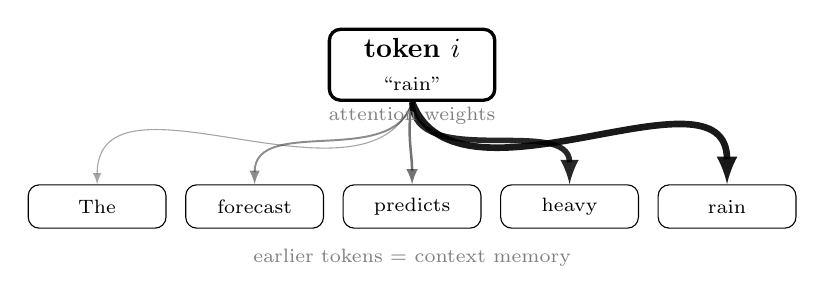
\begin{tikzpicture}[>=latex, x=1cm, y=1cm]

\tikzstyle{tok}=[draw, rounded corners, minimum width=1.75cm, minimum height=0.55cm, align=center]
\tikzstyle{qtok}=[draw, rounded corners, minimum width=2.1cm, minimum height=0.60cm, align=center, very thick]

% --- top: current token (query) ---
\node[qtok] (q) at (0,1.8) {\textbf{token $i$}\\{\scriptsize ``rain''}};

% --- bottom: context tokens (keys/values) ---
\node[tok] (t1) at (-4.0,0) {\scriptsize The};
\node[tok] (t2) at (-2.0,0) {\scriptsize forecast};
\node[tok] (t3) at ( 0.0,0) {\scriptsize predicts};
\node[tok] (t4) at ( 2.0,0) {\scriptsize heavy};
\node[tok] (t5) at ( 4.0,0) {\scriptsize rain};

% --- arrows = attention weights ---
\draw[->, line width=0.4pt, opacity=0.35] (q.south) to[out=250,in=90] (t1.north);
\draw[->, line width=0.7pt, opacity=0.45] (q.south) to[out=255,in=90] (t2.north);
\draw[->, line width=0.9pt, opacity=0.55] (q.south) to[out=260,in=90] (t3.north);
\draw[->, line width=2.0pt, opacity=0.85] (q.south) to[out=270,in=90] (t4.north);
\draw[->, line width=2.4pt, opacity=0.90] (q.south) to[out=290,in=90] (t5.north);

% --- labels ---
\node[align=center] at (0,1.15) {\scriptsize \textcolor{gray}{attention weights}};
\node[align=center] at (0,-0.65) {\scriptsize \textcolor{gray}{earlier tokens = context memory}};

\end{tikzpicture}
}

\end{frame}

%!TEX root = lec16.tex
% ================================================================================
% Lecture 16, Slide 11
% ================================================================================
\begin{frame}[t]
  \mytitle{Step 3: Training --- Next Token Prediction}

\begin{columns}[T,totalwidth=\textwidth]

% ------------------------------------------------------------
\begin{column}[T]{0.50\textwidth}
\footnotesize
\vspace{4mm}

\textbf{\textcolor{blue}{Training objective}}

\vspace{2mm}
\begin{itemize}
  \item show text to the model
  \item hide the next token
  \item train it to predict the hidden token
\end{itemize}

\vspace{3mm}
\textbf{\textcolor{red}{Result:}}
\quad the model learns grammar, style, facts, and reasoning patterns
\y{as an emergent capability}.

\vspace{3mm}
{\tiny
Important: training is expensive \\
(compute + data).  \\
Using a model is cheap (inference).
}

\end{column}

% ------------------------------------------------------------
\begin{column}[T]{0.46\textwidth}
\footnotesize
\vspace{4mm}

\textbf{\textcolor{violet}{Why it can fail}}

\vspace{2mm}
\begin{itemize}
  \item it predicts \textbf{plausible text}
  \item not guaranteed truth
  \item can \textbf{hallucinate} details
\end{itemize}

\vspace{3mm}
{\tiny \textcolor{gray}{
Therefore: verification + grounding are crucial in professional use.
}}
\end{column}

\end{columns}

% ------------------------------------------------------------
% Next token prediction visualization (TikZ)
% ------------------------------------------------------------
\vspace{-11mm}
\hspace*{4cm}
\scalebox{0.70}{
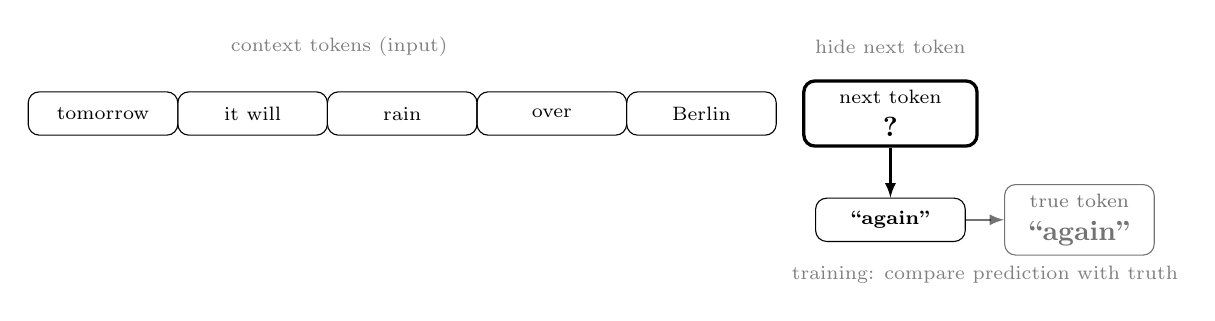
\begin{tikzpicture}[>=latex, x=1cm, y=1cm]

\tikzstyle{tok}=[draw, rounded corners, minimum width=1.9cm, minimum height=0.55cm, align=center]
\tikzstyle{tokfaint}=[draw, rounded corners, minimum width=1.9cm, minimum height=0.55cm, align=center, opacity=0.55]
\tikzstyle{tokspecial}=[draw, rounded corners, minimum width=2.2cm, minimum height=0.62cm, align=center, very thick]
\tikzstyle{arrow}=[->, thick]

% --- input tokens ---
\node[tok] (t1) at (-5.7,0) {\scriptsize tomorrow};
\node[tok] (t2) at (-3.8,0) {\scriptsize it will};
\node[tok] (t3) at (-1.9,0) {\scriptsize rain};
\node[tok] (t4) at ( 0.0,0) {\scriptsize over};
\node[tok] (t5) at ( 1.9,0) {\scriptsize Berlin};

% --- hidden next token ---
\node[tokspecial] (q) at (4.3,0) {\scriptsize next token\\\textbf{?}};

% --- model prediction ---
\node[tok] (pred) at (4.3,-1.35) {\scriptsize \textbf{``again''}};
\draw[arrow] (q.south) -- (pred.north);

% --- loss / training signal ---
\node[tokfaint] (true) at (6.7,-1.35) {\scriptsize true token\\\textbf{``again''}};
\draw[arrow, opacity=0.55] (pred.east) -- (true.west);

% --- captions ---
\node[align=center] at (-2.7,0.85) {\scriptsize \textcolor{gray}{context tokens (input)}};
\node[align=center] at (4.3,0.85) {\scriptsize \textcolor{gray}{hide next token}};
\node[align=center] at (5.5,-2.05) {\scriptsize \textcolor{gray}{training: compare prediction with truth}};

\end{tikzpicture}
}

\end{frame}

%!TEX root = lec16.tex
% ================================================================================
% Lecture 16, Slide 12
% ================================================================================
\begin{frame}[t]
  \mytitle{Inference: Prompting Is Steering}

\begin{columns}[T,totalwidth=\textwidth]

% ------------------------------------------------------------
\begin{column}[T]{0.50\textwidth}
\footnotesize
\vspace{0mm}

\textbf{\textcolor{blue}{A prompt creates the context}}

\vspace{0mm}
\begin{itemize}
  \item system message: role + rules
  \item user message: task + data
  \item the model continues from there
\end{itemize}

\vspace{4mm}
\textbf{\textcolor{red}{Key point:}}
\quad The model is \y{not stable by itself}.  
It is shaped by the context we provide.

\end{column}

% ------------------------------------------------------------
\begin{column}[T]{0.46\textwidth}
\footnotesize
\vspace{0mm}

\textbf{\textcolor{violet}{What improves results}}

\vspace{2mm}
\begin{itemize}
  \item clear goal + constraints
  \item examples of desired style
  \item provide trusted information
  \item ask for uncertainties / checks
\end{itemize}

\vspace{3mm}
{\tiny \textcolor{gray}{
Good prompting is a communication skill:
precise intent, good context, clear quality criteria.
}}
\end{column}

\end{columns}

% ------------------------------------------------------------
% Visualization: prompting = steering (TikZ)
% ------------------------------------------------------------
\vspace{0mm}
\begin{center}
\scalebox{0.85}{
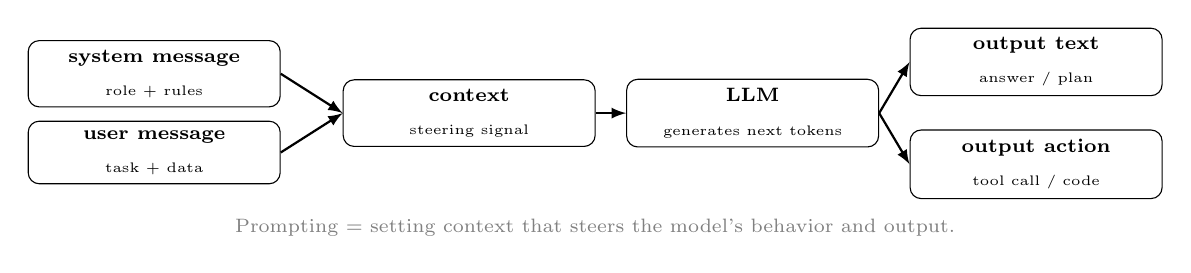
\begin{tikzpicture}[>=latex, x=1cm, y=1cm]

\tikzstyle{box}=[draw, rounded corners, minimum width=3.2cm, minimum height=0.8cm, align=center]
\tikzstyle{smallbox}=[draw, rounded corners, minimum width=3.2cm, minimum height=0.62cm, align=center]
\tikzstyle{arrow}=[->, thick]

% Left: system+user messages
\node[smallbox] (sys) at (-5.0,0.9) {\scriptsize \textbf{system message}\\{\tiny role + rules}};
\node[smallbox] (usr) at (-5.0,-0.1) {\scriptsize \textbf{user message}\\{\tiny task + data}};

% Middle: context / steering
\node[box] (ctx) at (-1.0,0.4) {\scriptsize \textbf{context}\\{\tiny steering signal}};

\draw[arrow] (sys.east) -- (ctx.west);
\draw[arrow] (usr.east) -- (ctx.west);

% Engine: model
\node[box] (llm) at (2.6,0.4) {\scriptsize \textbf{LLM}\\{\tiny generates next tokens}};

\draw[arrow] (ctx.east) -- (llm.west);

% Output
\node[smallbox] (out1) at (6.2,1.05) {\scriptsize \textbf{output text}\\{\tiny answer / plan}};
\node[smallbox] (out2) at (6.2,-0.25) {\scriptsize \textbf{output action}\\{\tiny tool call / code}};

\draw[arrow] (llm.east) -- (out1.west);
\draw[arrow] (llm.east) -- (out2.west);

% Small caption
\node[align=center] at (0.6,-1.05) {\scriptsize \textcolor{gray}{Prompting = setting context that steers the model's behavior and output.}};

\end{tikzpicture}
}
\end{center}

\end{frame}

%!TEX root = lec16.tex
% ================================================================================
% Lecture 16, Slide 13
% ================================================================================
\begin{frame}[t]
  \mytitle{From Language to Interaction: LLMs + Tools}

\begin{columns}[T,totalwidth=\textwidth]

% ------------------------------------------------------------
\begin{column}[T]{0.54\textwidth}
\footnotesize
\vspace{-1mm}

\textbf{\textcolor{blue}{LLMs become useful at work when connected}}

\vspace{-1mm}
\begin{itemize}\setlength{\itemsep}{1mm}

  \item \textbf{retrieval (RAG):} trusted documents
  {\tiny
  \begin{itemize}\setlength{\itemsep}{0mm}\setlength{\topsep}{0mm}\setlength{\parskip}{0mm}
    \item policies, manuals, guidance, internal knowledge bases
    \item reduces hallucinations by grounding on sources
  \end{itemize}
  }

  \item \textbf{tools:} APIs, code execution, search
  {\tiny
  \begin{itemize}\setlength{\itemsep}{0mm}\setlength{\topsep}{0mm}\setlength{\parskip}{0mm}
    \item from ``talking'' to \y{doing} (compute, query, automate)
    \item reproducible outputs: scripts, plots, tables
  \end{itemize}
  }

\end{itemize}

\vspace{-1mm}
\textbf{\textcolor{red}{Key message:}}
\quad Real systems are \y{LLM-based assistants}, not just chat.

\end{column}

% ------------------------------------------------------------
\begin{column}[T]{0.48\textwidth}
\centering
\vspace{-2mm}

\begin{itemize}
  \item \color{red}\textbf{memory:} project and user context
  {\tiny
  \begin{itemize}\setlength{\itemsep}{0mm}\setlength{\topsep}{0mm}\setlength{\parskip}{0mm}
    \item remembers assumptions, preferences, ongoing tasks
    \item avoids repeating the same onboarding every time
  \end{itemize}
  }
\end{itemize}

\includegraphics[width=\linewidth]{../../images/img16/rag.png}

\end{column}

\end{columns}

\end{frame}

%!TEX root = lec16.tex
% ================================================================================
% Lecture 16 — Slide 14
% ================================================================================
\begin{frame}[t,fragile]

\mytitle{From Chat to Action: Why Function Calling Matters}

\begin{columns}[T,totalwidth=\textwidth]

% ------------------------------------------------------------
\begin{column}[T]{0.48\textwidth}
\footnotesize

\vspace{6mm}
\textbf{Chat is not the goal.}

\vspace{2mm}
\rtext{\bf LLMs become truly useful when they can trigger \y{real actions}:}

\vspace{1mm}
\begin{itemize}
  \item download and inspect forecast data
  \item compute diagnostics and key numbers
  \item generate plots and reports
  \item call services (archives, NWP, HPC tools)
\end{itemize}

\vspace{2mm}
\textbf{Function calling} turns language into \y{structured decisions} ---
executed by a controlled backend (not by the LLM).

\end{column}

% ------------------------------------------------------------
\begin{column}[T]{0.5\textwidth}
\vspace{-2mm}

% --- tool call snippet ----------------------------------------------------------
{\scriptsize\textbf{Example: tool call proposed by the LLM}}
\vspace{1mm}

\tiny
\begin{lstlisting}
{
  "tool_name": "get_weather_forecast",
  "arguments": {
    "model": "ICON-EU",
    "variable": "t2m",
    "location": "Berlin",
    "lead_time_h": 24
  }
}
\end{lstlisting}

\vspace{-8mm}
% --- dawid icon-eu image --------------------------------------------------------
\begin{center}
\includegraphics[height=2cm]{../../images/img16/weather_reading_crop.png}

\vspace{2mm}
{\scriptsize \textit{DAWID executes the tool call and returns the result.}}
\end{center}

\end{column}

\end{columns}
\end{frame}

%!TEX root = lec16.tex
% ================================================================================
% Lecture 16 — Slide 15
% ================================================================================
\begin{frame}[t,fragile]
\mytitle{Tool Awareness: How the Model Knows What It Can Do}

\begin{columns}[T,totalwidth=\textwidth]

% ------------------------------------------------------------
\begin{column}[T]{0.48\textwidth}
\footnotesize
\vspace{2mm}

\textbf{The key idea}

\vspace{2mm}
The LLM cannot ``invent'' actions.
It can only call tools that we \rtext{explicitly provide}.

\vspace{2mm}
\textbf{Why this matters}
\begin{itemize}
  \item clear capabilities: \y{what is possible}
  \item safety boundary: \y{what is not allowed}
  \item reproducible results: same tool $\Rightarrow$ same behavior
\end{itemize}

\vspace{2mm}
\rtext{\textbf{Think of it as a menu:}
the model chooses an item, the system cooks it.}

\vspace{0mm}
\begin{center}
{\scriptsize \textit{The tool list becomes the model’s action space.}}
\end{center}

\end{column}

% ------------------------------------------------------------
\begin{column}[T]{0.52\textwidth}
\vspace{-2mm}

{\scriptsize\textbf{\y{Tool registry} (provided to the model)}}

\vspace{-3mm}
\tiny
\begin{lstlisting}
TOOLS = [
  {
    "name": "get_weather_forecast",
    "description": "Retrieve ICON-EU forecast values.",
    "inputs": {
      "location": "string",
      "variable": "t2m|wind|precip",
      "lead_time_h": "integer"
    }
  },
  {
    "name": "google_search",
    "description": "Search the web for up-to-date information and sources.",
    "inputs": { "query": "string" }
  }
]
\end{lstlisting}


\end{column}

\end{columns}
\end{frame}

%!TEX root = lec16.tex
% ================================================================================
% Lecture 16 — Slide 16
% ================================================================================
\begin{frame}[t]

\vspace{-3mm}
\begin{center}
\includegraphics[width=0.76\linewidth]{../../images/img16/function_or_agent_crop.png}
\end{center}


\end{frame}

\input{lec16_17.tex}
%!TEX root = lec16.tex
% ================================================================================
% Lecture 16 — Slide 18
% ================================================================================
\begin{frame}[t]
\mytitle{LLM Orchestration: Decisions \& Guardrails}

\begin{columns}[T,totalwidth=\textwidth]

% ------------------------------------------------------------
\begin{column}[T]{0.52\textwidth}
\footnotesize
\vspace{2mm}

\textbf{LLM = Decision Engine}

\vspace{2mm}
For each user request, the model decides \y{what happens next}:

\vspace{1mm}
\begin{itemize}
  \item answer directly (when trivial)
  \item call a function tool (fast action)
  \item delegate to an agent (multi-step work)
  \item ask a clarifying question (missing info)
\end{itemize}

\vspace{2mm}
\textbf{Key idea:}
The model routes the task to the best capability.

\vspace{1mm}
{\scriptsize \textit{(Like a dispatcher: choose the right action at the right time.)}}

\end{column}

% ------------------------------------------------------------
\begin{column}[T]{0.48\textwidth}
\footnotesize
\vspace{2mm}

\textbf{Guardrails = System Control}

\vspace{2mm}
The system stays in charge of \y{execution}:

\vspace{1mm}
\begin{itemize}
  \item only approved tools exist (tool registry)
  \item arguments are validated (schemas)
  \item execution runs outside the LLM
  \item logging \& reproducibility by design
\end{itemize}

\vspace{2mm}
\textbf{Result:}
Reliable actions, not hallucinated actions.

\vspace{1mm}
{\scriptsize \textit{The LLM proposes --- the backend disposes.}}

\end{column}

\end{columns}

\end{frame}

%!TEX root = lec16.tex
% ================================================================================
% Lecture 16 — Slide 19
% ================================================================================
\begin{frame}[t]
\mytitle{The Race for Function \& Agent Standards}

\begin{columns}[T,totalwidth=\textwidth]

% ------------------------------------------------------------
\begin{column}[T]{0.56\textwidth}
\footnotesize
\vspace{-2mm}

\textbf{OpenAI — Tool Calling + JSON Schema}
\begin{itemize}
  \item tools defined via \y{JSON Schema}
  \item \y{Structured Outputs / strict schema} for reliable calls
\end{itemize}

\vspace{2mm}
\textbf{Anthropic — MCP (Model Context Protocol)}
\begin{itemize}
  \item open connector: \y{model $\leftrightarrow$ MCP server $\leftrightarrow$ tools/data}
  \item goal: universal plug-in interface for enterprise tools
\end{itemize}

\vspace{2mm}
\includegraphics[width=0.45\linewidth]{../../images/img16/race01.png}
\includegraphics[width=0.45\linewidth]{../../images/img16/race02.png}

\end{column}

% ------------------------------------------------------------
\begin{column}[T]{0.44\textwidth}
\footnotesize
\vspace{-2mm}

\textbf{Google — Gemini Function Calling}
\begin{itemize}
  \item built-in function calling in the Gemini API ecosystem
  \item tight integration with the Google stack
\end{itemize}

\vspace{2mm}
\textbf{Linux Foundation / AAIF — Interoperability}
\begin{itemize}
  \item push for neutral/open \y{agent tool interfaces}
  \item avoid vendor lock-in and ``tool Babel''
\end{itemize}

\vspace{2mm}
\includegraphics[width=0.45\linewidth]{../../images/img16/race03.png}
\includegraphics[width=0.45\linewidth]{../../images/img16/race04.png}

\end{column}

\end{columns}
\end{frame}

%!TEX root = lec16.tex
% ================================================================================
% Lecture 16 — Slide 20
% ================================================================================
\begin{frame}[t]
\mytitle{Our Opportunity: DAWID Puts Trusted Functions at Our Fingertips}

\begin{columns}[T,totalwidth=\textwidth]

% ------------------------------------------------------------
\begin{column}[T]{0.52\textwidth}
\footnotesize
\vspace{-2mm}

\textbf{What we can do immediately}

\vspace{2mm}
DAWID gives us a practical advantage:
we can expose \y{our own operational capabilities} as tools.

\vspace{2mm}
\begin{itemize}
  \item tools = \y{trusted} ECMWF / DWD / NHMS \y{functions} (not generic chat)
  \item each tool encodes a workflow step we already know
  \item the LLM becomes the \y{orchestrator} and UI
\end{itemize}

\vspace{0mm}
\textbf{Result:}
\begin{itemize}
  \item faster exploration and analysis
  \item reproducible results (same tools, same outputs)
  \item knowledge transfer: tools carry expertise
\end{itemize}

\end{column}

% ------------------------------------------------------------
\begin{column}[T]{0.45\textwidth}

\vspace{-2mm}
\raggedleft
\includegraphics[width=5cm]{../../images/img16/fraim01}

\includegraphics[width=5.1cm]{../../images/img16/fraim02}

\vspace{1mm}
\centering
{\scriptsize \textit{DAWID: User Interface}}

\vspace{2mm}
\raggedleft
\rtext{\bf --- OUR functions!!}

\end{column}

\end{columns}
\end{frame}

%!TEX root = lec16.tex
% ================================================================================
% Lecture 16, Slide 14
% ================================================================================
\begin{frame}[t]
  \mytitle{AI Forecasting: Learning to Predict the Next Weather State}

\begin{columns}[T,totalwidth=\textwidth]

% ------------------------------------------------------------
\begin{column}[T]{0.5\textwidth}
\footnotesize
\vspace{2mm}

\textbf{\textcolor{blue}{Key idea}}

\vspace{2mm}
\begin{itemize}
  \item The atmosphere has a \textbf{state} (a snapshot)
  \item \y{Forecasting means predicting a \textbf{future state}}
  \item A neural network learns a mapping:
\end{itemize}

\vspace{2mm}
\[
x(t) \;\;\Rightarrow\;\; x(t+48h)
\]

\vspace{1mm}
{\tiny
where $x$ contains fields like temperature, wind, pressure, humidity.
}

\vspace{3mm}
\textbf{\textcolor{red}{Training:}}
\quad learn from millions of examples
(reanalysis + observations).

\vspace{2mm}
{\tiny
After training, the model can produce forecasts extremely fast.
}

\end{column}

% ------------------------------------------------------------
\begin{column}[T]{0.52\textwidth}

\centering
\vspace{1mm}
\includegraphics[width=0.7\linewidth]{../../images/img16/weather_t1_t48_rain_gsp_1honly_europe_crop.png}

\end{column}

\end{columns}
\end{frame}

%!TEX root = lec16.tex
% ================================================================================
% Lecture 16, Slide 15
% ================================================================================
\begin{frame}[t]
  \mytitle{Neural Network Forecasting: One Step $\rightarrow$ Many Steps}

\begin{columns}[T,totalwidth=\textwidth]

% ------------------------------------------------------------
\begin{column}[T]{0.48\textwidth}
\footnotesize
\vspace{1mm}

\textbf{\textcolor{blue}{How an AI forecast is produced}}

\vspace{2mm}
\begin{itemize}
  \item The model learns: \y{state now} $\rightarrow$ \y{state later}
  \item Longer lead times come from \textbf{repeating the prediction step}
\end{itemize}

\vspace{-2mm}
\[
x(t) \rightarrow x(t+\Delta t) \rightarrow x(t+2\Delta t) \rightarrow \dots
\]

\vspace{3mm}
\textbf{\textcolor{red}{Physics detail: accumulated variables}}

\vspace{1mm}
\begin{itemize}
  \item precipitation is often stored as an \textbf{accumulated sum}
  \item to get \textbf{1-hour rain} at lead $L$:
\end{itemize}

\vspace{-3mm}
\[
RAIN(L) - RAIN(L-1)
\]

\end{column}

% ------------------------------------------------------------
\begin{column}[T]{0.52\textwidth}
\centering
\vspace{1mm}

\includegraphics[width=\linewidth]{../../images/img16/rain_gsp_1h_2x4_panels_crop.png}

\vspace{1mm}
\textcolor{gray}{
Example: ICON-EU 1-hour precipitation for multiple lead times.
}

\vspace{3mm}
\rtext{\bf Here: Nowcasting or NWP - depending on input, time scales and variables!}
\end{column}

\end{columns}

\end{frame}

%!TEX root = lec16.tex
% ================================================================================
% Lecture 16, Slide 16
% ================================================================================
\begin{frame}[t]
  \mytitle{Nowcasting and NWP: One Continuum (Observations $\rightarrow$ DA $\rightarrow$ Forecast)}

\begin{columns}[T,totalwidth=\textwidth]

% ------------------------------------------------------------
\begin{column}[T]{0.52\textwidth}
\footnotesize
\vspace{2mm}

\textbf{\textcolor{blue}{NWP with Data Assimilation (DA) is the full framework}}

\vspace{0mm}
\begin{itemize}
  \item \textbf{observations} enter continuously:
    {\tiny \newline radar, satellite, aircraft, surface stations, etc.}
  \item \textbf{DA} combines obs + model:
    {\tiny \newline best estimate of the 3D atmosphere at ``now''}
  \item then \textbf{forecast propagation} produces future weather
\end{itemize}

\vspace{0mm}
\textbf{\textcolor{violet}{Nowcasting is the short-range regime}}

\vspace{1mm}
\begin{itemize}
  \item lead times: \textbf{minutes to a few hours}
  \item very high weight of recent observations
  \item focus on rapidly evolving phenomena:
    {\tiny \newline convective storms, precipitation cells}
\end{itemize}

\end{column}

% ------------------------------------------------------------
\begin{column}[T]{0.48\textwidth}
\centering
\vspace{2mm}

\includegraphics[width=\textwidth]{../../images/img16/nwc-to-fcst_crop.png}

\vspace{3mm}
{\tiny \textcolor{gray}{
AI can support different parts: observations, DA, model emulation, and products.
}}

\hspace*{-8mm}\y{There is no strict boundary: it is one continuum.}

\end{column}

\end{columns}

\end{frame}

%!TEX root = lec16.tex
% ================================================================================
% Lecture 16, Slide 17
% ================================================================================
\begin{frame}[t]
  \mytitle{Forecasting in One Sentence}

\begin{columns}[T,totalwidth=\textwidth]

% ------------------------------------------------------------
\begin{column}[T]{0.5\textwidth}
\footnotesize
\vspace{3mm}

\textbf{\textcolor{blue}{Weather forecasting = state estimation + prediction}}

\vspace{2mm}
\begin{itemize}
  \item We estimate the \textbf{current atmospheric state}
  \item Then we predict how it changes in time
\end{itemize}

\vspace{-2mm}
\[
\underbrace{x(t_0)}_{\text{best estimate now}}
\quad \rightarrow \quad
\underbrace{x(t_0+\Delta t)}_{\text{future state}}
\]

\vspace{3mm}
\textbf{\textcolor{red}{Why it is hard}}

\vspace{1mm}
\begin{itemize}
  \item the atmosphere is \textbf{chaotic}
  \item small errors grow with time
  \item observations are incomplete and noisy
\end{itemize}

\end{column}

% ------------------------------------------------------------
\begin{column}[T]{0.5\textwidth}

\vspace{-5mm}
\textbf{\textcolor{violet}{So we quantify uncertainty}}
\begin{itemize}
  \item ensembles: many forecasts instead of one
\end{itemize}

\centering
\vspace{2mm}

% image placeholder (you can replace)
\includegraphics[width=\linewidth]{../../images/img16/nwp_continuum_crop.png}

\vspace{1mm}
{\tiny \textcolor{gray}{Forecasting: observation $\rightarrow$ analysis $\rightarrow$ prediction}}
\end{column}

\end{columns}

\end{frame}

%!TEX root = lec16.tex
% ================================================================================
% Lecture 16, Slide 18
% ================================================================================
\begin{frame}[t]
\centering
\vspace{-2mm}

\includegraphics[width=0.8\linewidth]{../../images/img16/nwp_neural.png}

\end{frame}

%!TEX root = lec16.tex
% ================================================================================
% Lecture 16, Slide 19
% ================================================================================
\begin{frame}[t]
  \mytitle{How a Neural Network Learns Forecasting: Front Template + Motion}

\centering
\vspace{-2mm}

\includegraphics[width=0.6\linewidth]{../../images/img16/nn_front_visual_argument_4panel.png}

\vspace{1mm}
{\footnotesize \textcolor{gray}{
Visual argument: the NN learns \textbf{templates} (front patterns) and how they
\textbf{move / evolve} over time.
}}

\end{frame}

%!TEX root = lec16.tex
% ================================================================================
% Lecture 16, Slide 20
% ================================================================================
\begin{frame}[t]
  \mytitle{One Step, Many Steps: Templates + Transport + Accumulations}

\begin{columns}[T,totalwidth=\textwidth]

% ------------------------------------------------------------
\begin{column}[T]{0.48\textwidth}
\footnotesize
\vspace{0mm}

\textbf{\textcolor{blue}{Neural forecasting learns reusable building blocks}}

\vspace{1mm}
\begin{itemize}
  \item learn \textbf{templates} for structures:
    {\tiny \newline fronts, rain bands, vortices, jets}
  \item learn \textbf{how they move and change} from context
    {\tiny \newline (e.g. wind, humidity, stability)}
\end{itemize}

\vspace{0mm}
\textbf{\textcolor{blue}{Then: one step $\rightarrow$ many steps}}

\vspace{-2mm}
\[
x(t) \rightarrow x(t+\Delta t) \rightarrow x(t+2\Delta t) \rightarrow \dots
\]

\vspace{0mm}
\textbf{\textcolor{red}{Important for users: accumulated products}}

\vspace{1mm}
\begin{itemize}
  \item many outputs are stored as \textbf{accumulations}
  \item 1-hour precipitation at lead $L$ is:
\end{itemize}

\end{column}

% ------------------------------------------------------------
\begin{column}[T]{0.48\textwidth}

\vspace{1mm}
\[
RAIN(L) - RAIN(L-1)
\]

\vspace{0mm}
\textbf{\textcolor{violet}{Take-away:}}
\quad \y{Forecasting = detect patterns +} \\
\hfill \y{transport them forward in time.}


\centering
\vspace{4mm}

\includegraphics[width=\linewidth]{../../images/img16/nn_front_template_motion.png}

\vspace{1mm}
{\tiny \textcolor{gray}{
Templates $\rightarrow$ heatmaps $\rightarrow$ shifted patterns $\rightarrow$ next map
(repeated for longer lead times).
}}
\end{column}

\end{columns}

\end{frame}

%!TEX root = lec16.tex
% ================================================================================
% Lecture 16 — Slide 28
% ================================================================================
\begin{frame}[t]
\mytitle{A Minimal Forecasting World: A Blob Moving on a Circle}

\begin{columns}[T,totalwidth=\textwidth]

% ------------------------------------------------------------
\begin{column}[T]{0.52\textwidth}
\footnotesize

\vspace{4mm}
We create a simple 1D world on $[0,10]$:

\vspace{1mm}
\begin{itemize}
  \item a \y{function} $f(t,x)$ (a ``blob'')
  \item periodic domain: $x=0$ connects to $x=10$
  \item dynamics: \y{pure translation}
  \[
  f(t+\Delta,x) = f(t,x-\delta)
  \]
\end{itemize}

\vspace{2mm}
\textbf{Forecasting task:}
given $f(t,\cdot)$, predict $f(t+\Delta,\cdot)$.

\vspace{2mm}
This captures the essence of advection:
\y{structures move}.

\end{column}

% ------------------------------------------------------------
\begin{column}[T]{0.48\textwidth}

\vspace{-6mm}
\begin{center}
\includegraphics[width=\linewidth]{../../images/img16/cnn_translation_input_output.png}

\vspace{1mm}
{\scriptsize \textit{Input $f(t)$ and target/forecast $f(t+\Delta)$.}}

\vspace{-8mm}
\includegraphics[width=5cm]{../../images/img16/signal_on_circle_3d_crop.png}

\end{center}
\end{column}

\end{columns}
\end{frame}

%!TEX root = lec16.tex
% ================================================================================
% Lecture 16 — Slide 29
% ================================================================================
\begin{frame}[t]
\mytitle{What the Neural Network Sees}

\begin{columns}[T,totalwidth=\textwidth]

% ------------------------------------------------------------
\begin{column}[T]{0.5\textwidth}
\footnotesize
\vspace{-2mm}

\textbf{Important: the input is the \y{full signal}, not single points.}

\vspace{1mm}
The network gets all grid values of $f(t,x)$ at once:
\[
f(t,\cdot)\in\mathbb{R}^{N}\qquad (N=256)
\]

\vspace{2mm}
\textbf{But the computation is local:}
each output point is computed from a \y{neighborhood}.

\vspace{6mm}
\textbf{Kernel size $k$ = width of the filter}

\vspace{1mm}
With $k=7$, the network looks at:
\[
[x_{i-3},\dots,x_i,\dots,x_{i+3}]
\]

\end{column}

% ------------------------------------------------------------
\begin{column}[T]{0.44\textwidth}

\vspace{-6mm}
\textbf{Stacking layers increases context}

\vspace{1mm}
After 3 conv layers (all $k=7$), each output point depends on roughly:
\[
1 + 3\cdot(k-1) = 19\ \text{grid points}
\]

\hspace*{-1cm}\includegraphics[height=4cm]{../../images/img16/cnn_layers_influence.png}

\end{column}

\end{columns}
\end{frame}

%!TEX root = lec16.tex
% ================================================================================
% Lecture 16 — Slide 30
% ================================================================================
\begin{frame}[t]
\mytitle{Inside the CNN: Many Feature Variables}

\begin{columns}[T,totalwidth=\textwidth]

% ------------------------------------------------------------
\begin{column}[T]{0.44\textwidth}
\footnotesize
\vspace{-2mm}

The CNN transforms the input into many internal variables:

\vspace{2mm}
\begin{center}
{\Large $1 \rightarrow 32 \rightarrow 32 \rightarrow 32 \rightarrow 1$}
\end{center}

\vspace{2mm}
\begin{itemize}
  \item input: one function $f(t,x)$
  \item hidden layers: 32 feature channels each
  \item output: predicted function $\hat f(t+\Delta,x)$
\end{itemize}

\vspace{2mm}
\textbf{Interpretation:}
each channel is a learned detector for local shapes
(edges, slopes, curvature, \dots).

\end{column}

% ------------------------------------------------------------
\begin{column}[T]{0.48\textwidth}
\vspace{-8mm}
\begin{center}
\includegraphics[width=\linewidth]{../../images/img16/cnn_translation_features_h1.png}

\vspace{1mm}
{\scriptsize \textit{Example: 6 of 32 feature channels in layer $h1$.}}
\end{center}

\hspace{-12mm}
\begin{minipage}{7.5cm}
\footnotesize
The variables $h_1,h_2,h_3$ are \y{hidden feature maps} inside the CNN.
They form a \y{latent feature space}: not observed, not physical, but learned.
Each layer contains many channels (e.g.\ 32), extracting different local aspects of the signal.
The forecast emerges by transforming $f(t,\cdot)\rightarrow h_1\rightarrow h_2\rightarrow h_3\rightarrow \hat f(t+\Delta,\cdot)$.
\end{minipage}

\end{column}

\end{columns}
\end{frame}

%!TEX root = lec16.tex
% ================================================================================
% Lecture 16 — Slide 31
% ================================================================================
\begin{frame}[t]
\mytitle{Why This Is \emph{Not} Explicit Pattern Matching}

\begin{columns}[T,totalwidth=\textwidth]

% ------------------------------------------------------------
\begin{column}[T]{0.56\textwidth}
\footnotesize
\vspace{-2mm}

A common misconception is:
\begin{center}
\textit{``The network finds the blob pattern and just copies it forward.''}
\end{center}

\vspace{2mm}
\textbf{What actually happens:}
\begin{itemize}
  \item the CNN computes many internal feature variables (32 channels)
  \item each channel responds to \y{different local aspects}
  \item the forecast is produced by recombining these features
\end{itemize}

\vspace{2mm}
\rtext{\textbf{Key point:}
the NN does not store templates --- it learns a \y{continuous mapping}
from input to forecast.}

\end{column}

% ------------------------------------------------------------
\begin{column}[T]{0.44\textwidth}

\vspace{-8mm}
\begin{center}
\includegraphics[width=\linewidth]{../../images/img16/cnn_translation_features_h2.png}
\includegraphics[width=\linewidth]{../../images/img16/cnn_translation_features_h3.png}

\vspace{1mm}
{\scriptsize \textit{Example: 6 of 32 feature channels in layer $h3$.}}
\end{center}
\end{column}

\end{columns}
\end{frame}

%!TEX root = lec16.tex
% ================================================================================
% Lecture 16 — Slide XX
% ================================================================================
\begin{frame}[t]
\mytitle{What We Can Do Already}

\begin{columns}[T,totalwidth=\textwidth]

% ------------------------------------------------------------
\begin{column}[T]{0.46\textwidth}
\vspace{-2mm}

\begin{center}
\includegraphics[width=\linewidth]{../../images/img16/earth_forecast2.png}
\end{center}

\textbf{We already have strong building blocks in place:}

\vspace{2mm}
\begin{itemize}
  \item We have created a \y{framework} \y{for AI-based} \y{weather forecasting}
  with \rtext{Anemoi}
\end{itemize}

\end{column}

% ------------------------------------------------------------
\begin{column}[T]{0.56\textwidth}
\footnotesize
\vspace{-10mm}

\begin{itemize}
  \item We have developed libraries (\rtext{mfai, FRAIM}) for:
  \begin{itemize}
    \item \y{downscaling} and high-resolution products 
    \item \y{road weather} services
    \item high-impact weather \y{feature extraction}
    \item weather \y{interpretation} and \y{explainability}
    \item \y{nowcasting} of observation fields (radiation, precipitation, \dots)
  \end{itemize}
  
  \vspace{3mm}\color{darkgreen}
  \item We have gained expertise across the full \y{AI/ML value chain}
        in weather services and international organizations.
  \item \color{red} We have created \y{networking and structures} for joint development
        and sustainable research --- connected to leading global AI/ML developments.
\end{itemize}

\end{column}

\end{columns}
\end{frame}

%!TEX root = lec16.tex
% ================================================================================
% Lecture 16 — Slide XX
% ================================================================================
\begin{frame}[t]
\mytitle{What We Can Do Already (Operational AI Forecasting)}

\begin{columns}[T,totalwidth=\textwidth]

% ------------------------------------------------------------
\begin{column}[T]{0.58\textwidth}
\footnotesize
\vspace{-2mm}

\textbf{AI forecasting is already operational.}

\vspace{0mm}
In Europe, several AI-based forecasting systems are now in \y{production use} 
(e.g. AIFS, AICON, BRIS).
They complement classical NWP by providing:
\begin{itemize}
  \item fast state-to-state forecasts (minutes instead of hours)
  \item competitive large-scale skill for key variables
  \item robust baselines and rapid experimentation
\end{itemize}

\vspace{0mm}
\textbf{Key message:}
AI is no longer ``research only'' --- it is \y{part of the operational toolbox}.

\vspace{2mm}
This opens a clear opportunity:
\begin{itemize}
  \item combine NWP + AI hybrids
  \item integrate new observation-driven products 
  \item accelerate development cycles via ML pipelines
\end{itemize}

\end{column}

% ------------------------------------------------------------
\begin{column}[T]{0.42\textwidth}
\vspace{-3mm}

\begin{center}
\includegraphics[width=0.7\linewidth]{../../images/img16/already1.png}

\vspace{2mm}
\includegraphics[width=0.5\linewidth]{../../images/img16/already2.png}

\vspace{2mm}
\includegraphics[width=0.7\linewidth]{../../images/img16/already3.png}
\end{center}

\end{column}

\end{columns}
\end{frame}

%!TEX root = lec16.tex
% ================================================================================
% Lecture 16 — Slide XX
% ================================================================================
\begin{frame}[t]
\mytitle{Library Ecosystem: Complementary Capabilities}

\begin{columns}[T,totalwidth=\textwidth]

% ------------------------------------------------------------
\begin{column}[T]{0.52\textwidth}
\footnotesize
\vspace{-2mm}

\textbf{We are building a strong ecosystem of AI libraries}

\vspace{0mm}
Different libraries contribute complementary capabilities:
\begin{itemize}
  \item \textbf{Anemoi:} end-to-end AI weather models 
  \item \textbf{mfai:} vision transformers and many applications
  \item \textbf{MLCast:} nowcasting library, observation based
  \item \textbf{FRAIM:} products and services, full value chain
\end{itemize}

\vspace{0mm}
\textbf{Positive outlook}
\begin{itemize}
  \item no single library needs to do everything
  \item modular building blocks enable rapid innovation
  \item shared standards $\Rightarrow$ interoperability and reuse
\end{itemize}

\vspace{0mm}
\rtext{\textbf{Key message:}
Together, these components form a \y{platform for scalable AI in weather services}.}

\end{column}

% ------------------------------------------------------------
\begin{column}[T]{0.48\textwidth}
\vspace{-2mm}
\begin{center}
\includegraphics[width=\linewidth]{../../images/img16/library_ecosystem2.png}

\vspace{1mm}
{\scriptsize \textit{Ecosystem view: different strengths, one common mission.}}
\end{center}
\end{column}

\end{columns}
\end{frame}

%!TEX root = lec16.tex
% ================================================================================
% Lecture 16 — Slide 35
% ================================================================================
\begin{frame}[t]
\mytitle{Why Physics Matters: Future AI Forecast Systems Will Be \rtext{Physics + AI}}

\begin{columns}[T,totalwidth=\textwidth]

% ------------------------------------------------------------
\begin{column}[T]{0.52\textwidth}
\footnotesize
\vspace{-2mm}

\textbf{Weather is not just a pattern problem}

\vspace{0mm}
Forecasting is about \y{consistent evolution} of a \y{physical state}:
\begin{itemize}
  \item conservation laws (mass, energy, water)
  \item balances and constraints (geostrophy, stability)
  \item multiscale interactions (local storms $\leftrightarrow$ global flow)
\end{itemize}

\vspace{0mm}
\textbf{Why ``pure AI'' can fail}
\begin{itemize}
  \item excellent short-term skill can still drift long-term
  \item small violations accumulate (mass / moisture / energy)
  \item rare extremes need physics consistency, not just averages
\end{itemize}

\end{column}

% ------------------------------------------------------------
\begin{column}[T]{0.48\textwidth}

\vspace{-4mm}
\begin{center}
\includegraphics[width=\linewidth]{../../images/img16/earth_forecast2.png}

\vspace{0mm}
{\scriptsize \rtext{\textbf{AI gives speed and learning. \\
Physics gives truth and trust.}}}
\end{center}

\vspace{-2mm}\color{darkgreen}
\begin{itemize}
  \item AI learns \y{corrections / closures}
  \item constraints and invariants built \y{into the model}
  \item physics-based evaluation \& reliability
\end{itemize}

\end{column}

\end{columns}
\end{frame}

%!TEX root = lec16.tex
% ================================================================================
% Lecture 16 — Slide 36
% ================================================================================
\begin{frame}[t]
\mytitle{What You Can Do (A): Use LLMs as a Tool --- You Stay the Master}

\begin{columns}[T,totalwidth=\textwidth]

% ------------------------------------------------------------
\begin{column}[T]{0.56\textwidth}
\footnotesize
\vspace{-2mm}

\textbf{Use AI for: understanding, exploring, developing}

\vspace{1mm}
Think of LLMs as a \y{power tool} for knowledge work:
\begin{itemize}
  \item explain unfamiliar concepts in your context
  \item explore alternatives and trade-offs quickly
  \item generate drafts, code sketches, slide structure
  \item summarize documents, meetings, research threads
\end{itemize}

\vspace{2mm}
\textbf{The right mindset}
\begin{itemize}
  \item \y{you are the pilot}, the AI is the assistant
  \item ask for options, then decide yourself
  \item validate important facts (sources, experiments)
\end{itemize}

\vspace{2mm}
\rtext{\textbf{Key message:}}
AI needs guidance --- quality comes from \y{your questions and your checks}.

\end{column}

% ------------------------------------------------------------
\begin{column}[T]{0.44\textwidth}

\vspace{-6mm}
\begin{center}
\includegraphics[width=\linewidth]{../../images/img16/ai_books.png}

\vspace{-3mm}
{\scriptsize \rtext{\textbf{Human judgment stays in control.}}}
\end{center}
\end{column}

\end{columns}
\end{frame}

%!TEX root = lec16.tex
% ================================================================================
% Lecture 16 — Slide 37
% ================================================================================
\begin{frame}[t]
\mytitle{What LLMs Do Today --- and What ``World Models'' Add Next}

\begin{columns}[T,totalwidth=\textwidth]

% ------------------------------------------------------------
\begin{column}[T]{0.54\textwidth}
\footnotesize
\vspace{-2mm}

\textbf{LLMs today (what they actually do)}
\begin{itemize}
  \item generate text/code by \y{next-token prediction}
  \item strong at language tasks: explain, summarize, draft, transform
  \item can \y{appear} to reason, but truth not guaranteed
  \item without grounding: can be \rtext{confidently wrong}
\end{itemize}

\vspace{2mm}
\tiny
\textbf{World-model approaches (the next step)}
\begin{itemize}
  \item learn explicit \y{state} representations of a system (world state)
  \item learn \y{dynamics}: state$(t)$ + action $\rightarrow$ state$(t{+}1)$
  \item enable planning, long-horizon consistency, and controllable actions
  \item usually needs \y{grounding} (data, sensors, simulators, tools)
\end{itemize}

\vspace{0mm}
\footnotesize
\rtext{\textbf{Message:}}
LLMs are powerful interfaces --- world models aim at \y{reliable dynamics}.

\end{column}

% ------------------------------------------------------------
\begin{column}[T]{0.44\textwidth}
\footnotesize
\vspace{-2mm}

\textbf{LLMs for knowledge work}

\tiny
\vspace{0mm}\color{red}
\textbf{Be careful:}
\begin{itemize}\color{darkgreen}
  \item verify facts, numbers, and operational details
  \item demand sources or reproduce with scripts
  \item watch for missing assumptions and edge cases
\end{itemize}

\footnotesize
\vspace{0mm}
\textbf{Take full advantage:}
\begin{itemize}
  \item accelerate understanding and documentation
  \item structure tasks into steps, checklists, and options
  \item generate first drafts and improve clarity
  \item connect to tools/agents for \y{grounded actions}
\end{itemize}

\vspace{-1mm}
\rtext{\textbf{Fast thinking + human validation \\
= real productivity.}}

\end{column}

\end{columns}
\end{frame}

%!TEX root = lec16.tex
% ================================================================================
% Lecture 16 — Slide 38
% ================================================================================
\begin{frame}[t]
\mytitle{What You Can Do (B): Rebuild Services with Tools, Agents, and Clear APIs}

\begin{columns}[T,totalwidth=\textwidth]

% ------------------------------------------------------------
\begin{column}[T]{0.58\textwidth}
\footnotesize
\vspace{-2mm}

\textbf{Use the AI revolution to modernize services}

\vspace{0mm}
LLMs work best when they can call \y{clear interfaces}.
This is an opportunity to rebuild our services in a clean way:

\vspace{0mm}
\begin{itemize}
  \item define small, robust \y{functions} (tools)
  \item combine them into \y{agent workflows}
  \item expose everything as \y{API-based services}
\end{itemize}

\vspace{0mm}
\textbf{Why this is powerful}
\begin{itemize}
  \item clarity: inputs/outputs become explicit
  \item reuse: one tool serves many applications
  \item automation: agents connect tools: end-to-end
  \item acceleration: faster prototyping and delivery
\end{itemize}

\vspace{0mm}
\rtext{\textbf{Key message:}}
LLMs need good tool definitions --- \y{we can use this to create better services for ourselves.}

\end{column}

% ------------------------------------------------------------
\begin{column}[T]{0.42\textwidth}
\vspace{-2mm}
\begin{center}
\includegraphics[width=\linewidth]{../../images/img16/function_or_agent_crop.png}

\vspace{1mm}
{\scriptsize \textit{Tool calling turns services into reusable building blocks.}}
\end{center}
\end{column}

\end{columns}
\end{frame}

%!TEX root = lec16.tex
% ================================================================================
% Lecture 16 — Slide 39
% ================================================================================
\begin{frame}[t]
\mytitle{Slide 39: Rebuild Services --- Analyze Work, Find Waste, Build Tools}

\begin{columns}[T,totalwidth=\textwidth]

% ------------------------------------------------------------
\begin{column}[T]{0.50\textwidth}
\footnotesize
\vspace{-2mm}

\textbf{Step 1: Look at our daily workflow}
\begin{itemize}
  \item Where do we \rtext{repeat} the same steps?
  \item Where do we \rtext{copy/paste} between systems?
  \item Where do we \rtext{wait} for data, plots, approvals?
  \item Where do we \rtext{lose context} (emails, chats, files)?
\end{itemize}

\vspace{2mm}
\textbf{Step 2: Turn waste into tools}
\begin{itemize}
  \item define a clear \y{input/output interface}
  \item make it callable (API / function / agent tool)
  \item reuse it everywhere: DAWID, scripts, services, pipelines
\end{itemize}

\end{column}

% ------------------------------------------------------------
\begin{column}[T]{0.50\textwidth}
\vspace{-2mm}

\begin{center}
\scalebox{0.6}{
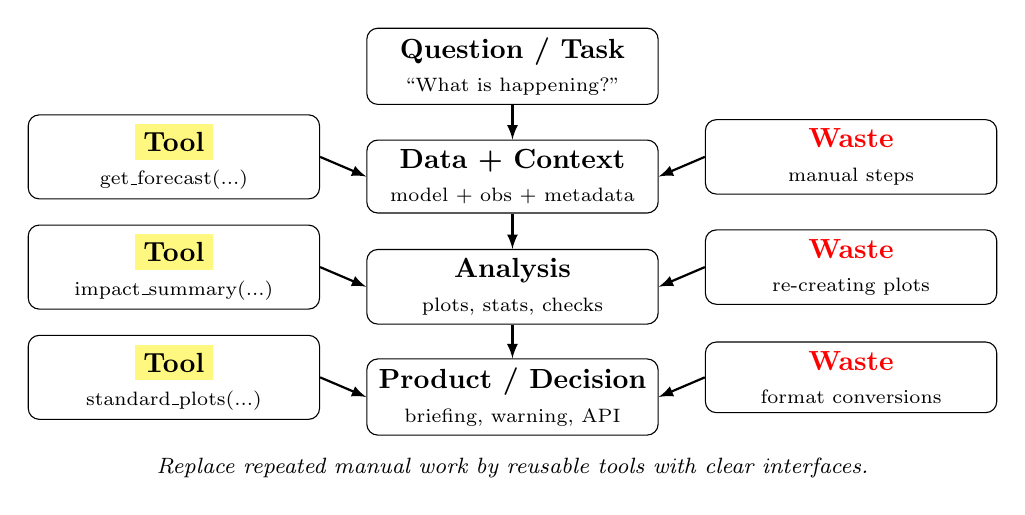
\begin{tikzpicture}[x=1cm,y=1cm,>=latex]

\tikzstyle{box}=[draw,rounded corners,align=center,minimum width=3.7cm,minimum height=0.85cm]
\tikzstyle{waste}=[draw,rounded corners,align=center,minimum width=3.7cm,minimum height=0.75cm]
\tikzstyle{tool}=[draw,rounded corners,align=center,minimum width=3.7cm,minimum height=0.75cm]
\tikzstyle{arrow}=[->,thick]

% ------------------------------------------------------------
% main chain (more vertical spacing)
% ------------------------------------------------------------
\node[box] (q) at (0,4.2) {\textbf{Question / Task}\\{\scriptsize ``What is happening?''}};
\node[box] (d) at (0,2.8) {\textbf{Data + Context}\\{\scriptsize model + obs + metadata}};
\node[box] (a) at (0,1.4) {\textbf{Analysis}\\{\scriptsize plots, stats, checks}};
\node[box] (p) at (0,0.0) {\textbf{Product / Decision}\\{\scriptsize briefing, warning, API}};

\draw[arrow] (q) -- (d);
\draw[arrow] (d) -- (a);
\draw[arrow] (a) -- (p);

% ------------------------------------------------------------
% waste tags on the right (aligned to chain)
% ------------------------------------------------------------
\node[waste] (w1) at (4.3,3.05) {\rtext{\textbf{Waste}}\\{\scriptsize manual steps}};
\node[waste] (w2) at (4.3,1.65) {\rtext{\textbf{Waste}}\\{\scriptsize re-creating plots}};
\node[waste] (w3) at (4.3,0.25) {\rtext{\textbf{Waste}}\\{\scriptsize format conversions}};

\draw[arrow] (w1.west) -- (d.east);
\draw[arrow] (w2.west) -- (a.east);
\draw[arrow] (w3.west) -- (p.east);

% ------------------------------------------------------------
% tools on the left (aligned to chain)
% ------------------------------------------------------------
\node[tool] (t1) at (-4.3,3.05) {\y{\textbf{Tool}}\\{\scriptsize get\_forecast(...)}};
\node[tool] (t2) at (-4.3,1.65) {\y{\textbf{Tool}}\\{\scriptsize impact\_summary(...)}};
\node[tool] (t3) at (-4.3,0.25) {\y{\textbf{Tool}}\\{\scriptsize standard\_plots(...)}};

\draw[arrow] (t1.east) -- (d.west);
\draw[arrow] (t2.east) -- (a.west);
\draw[arrow] (t3.east) -- (p.west);

% ------------------------------------------------------------
% small caption
% ------------------------------------------------------------
\node[align=center] at (0,-0.9) {\footnotesize \textit{Replace repeated manual work by reusable tools with clear interfaces.}};

\end{tikzpicture}
}
\end{center}

\end{column}

\end{columns}

\vspace{2mm}
\rtext{\textbf{Key message:}}
If a task repeats, it should become a \y{tool}.

\end{frame}

%!TEX root = lec16.tex
% ================================================================================
% Lecture 16 — Slide XX
% ================================================================================
\begin{frame}[t]
\mytitle{What You Can Do (C): Bring Your Domain Expertise --- Make AI Your Own}

\begin{columns}[T,totalwidth=\textwidth]

% ------------------------------------------------------------
\begin{column}[T]{0.54\textwidth}
\footnotesize
\vspace{-2mm}

\textbf{AI becomes powerful when it is grounded in meteorology}

\vspace{0mm}
LLMs and neural networks do not automatically understand:
\begin{itemize}
  \item processes, states, and transitions
  \item limits and plausibility
  \item physical constraints and balances
  \item weather regimes and rare extremes
\end{itemize}

\vspace{2mm}\color{blue}
\textbf{Your expertise is the missing ingredient}
\begin{itemize}\color{blue}
  \item define what matters: variables, events, diagnostics
  \item define what is allowed: limits, physics, consistency
  \item define what is useful: products, warnings, explanations
\end{itemize}


\end{column}

% ------------------------------------------------------------
\begin{column}[T]{0.42\textwidth}

\vspace{0mm}
\rtext{\textbf{Key message:}}
Do not outsource AI --- \y{embed your knowledge} 
into tools, workflows, and constraints.

\vspace{2mm}
\begin{center}
\includegraphics[width=\linewidth]{../../images/img16/physics_and_ai.png}

\vspace{-1mm}
{\scriptsize \rtext{\textbf{Domain expertise turns AI into trust.}}}
\end{center}
\end{column}

\end{columns}
\end{frame}



% --- End Document ---------------------------------------------------------------
\end{document}
